\chapter{Introduction}
\label{chap:introduction}
Humans, from time immemorial, have looked at the earth and seen things interacting with each other; they have looked at the skies and wondered what the stars and planets were; they have looked at each other and invented communication, co-operation, society, and culture.
The process of observing the world and understanding these observations is arguably still the way we reason about the world.
Ever since the democratization of cameras, the process of reasoning about visual observations has become computational.
% Camera technology has made that process of reasoning about wa computational one.
The pursuit of developing such computations \textit{is} computer vision.
When the outputs of the reasoning process convey meaningful concepts to humans, we shall call it semantic visual understanding.

This introductory chapter is designed to be a bird's-eye-view of semantic visual understanding.
First, I will introduce a hierarchy of computer vision tasks that allows us to separate semantics from physics.
Second, I will briefly revisit the progress made in prototypical computer vision tasks and the benchmarks and datasets that have been established by researchers over the years for these tasks.
Third, we will discuss the implications of recent successes in computer vision and motivate the core ideas of this thesis along with an outline.
This will lay the groundwork for the rest of this dissertation.
Chapter \ref{chap:background} is meant to be a technical treatment of the background, related work, and existing methodologies for robust visual understanding.

\section{Understanding What Cameras See} 
\begin{figure}[t]
    \centering
    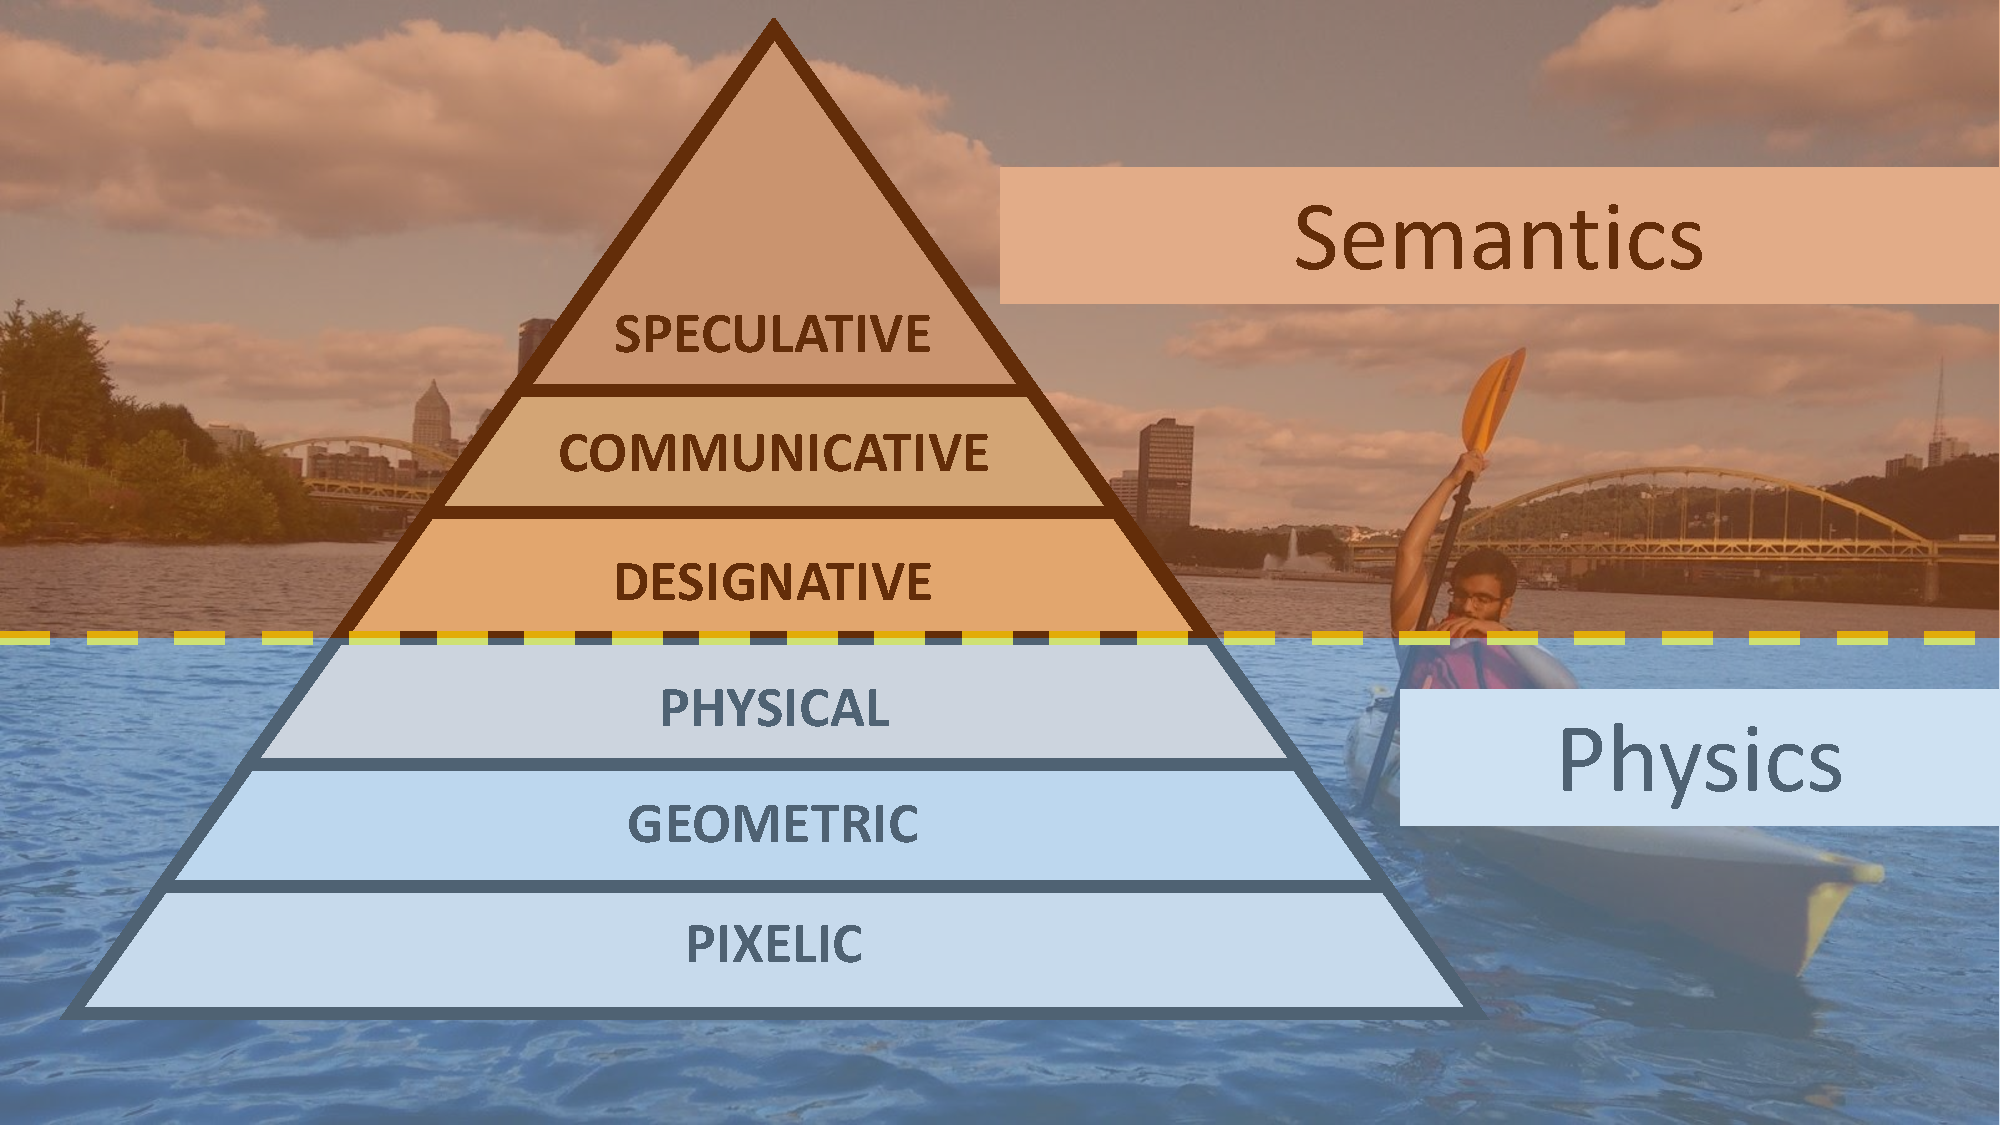
\includegraphics[width=\linewidth]{figures/visual_understanding_pyramid.pdf}
    \caption{A pyramidal hierarchy of visual understanding. This thesis largely deals with semantic vision, especially designative and communicative aspects of semantic vision.}
    \label{fig:visual_understanding_pyramid}
\end{figure}
While computer vision traces its roots and shares many of the goals of digital image processing~\citep{rosenfeld1976digital}, in the 1970s, computer vision underwent a paradigm shift.
While image processing was more focused on developing algorithms for acquisition, storage and information extraction from images, computer vision researchers are motivated by a larger goal -- to \textit{recover} information about scenes that is lost when an image is captured by a camera.
This includes \textit{``pixelic''} analysis such as edge detection and color detection; \textit{``geometric''} properties of the scene, for instance, three-dimensional properties such as depth, surface normals, orientation, and shape; and \textit{``physical''} properties of the scene such as estimating material reflectances, albedo, texture, etc. 
Computer vision also seeks to understand what objects (such as people, boats, trees, bridges, buildings) are present in an image, and where (localization). I call this category of vision, \textit{``designative''} vision since the aim is to designate or assign names and categorical labels to the observed visual input.
More recently, computer vision has also begun to serve in a \textit{``communicative''} role, for instance, the task of learning captions for images~\citep{yang2011corpus,karpathy2015deep} allows computer vision algorithms to express the scene in a human-understandable format.
Similarly, visual question answering~\citep{antol2015vqa} enable users to ask questions about the image and get answers from the computer vision system.
There has also been interest in \textit{``speculative''} vision, sometimes also controversially referred to as ``commonsense''~\citep{zellers2019recognition,park2020visualcomet} in literature; the aim is to speculate about intentions of people, their relationship with each other or with other objects, to speculate about their past or future actions and the effect of these actions, or to reason about why those actions are being performed.

Figure~\ref{fig:visual_understanding_pyramid} summarizes this hierarchy of visual understanding into six broad categories, and divides this spectrum into two main parts -- semantic vision and physics-based vision.
\textit{This thesis focuses on semantic vision.}


\section{Recent Success In Visual Understanding}
The fabled memo-meme from the 1950s to ``solve'' computer vision as a summer project ~\citep{papert1966summer} has grown as one of the biggest and most active research programs of scientific research in recent years~\citep{su2021affective}.
Computer vision occupies a large role in the popularity and applicability of machine learning algorithms.
Several standards benchmarks have been established, adopted, and celebrated by the community for many vision tasks.
Below, I will briefly review progress made on some of these datasets which lie in the category of \textit{``designative''} and \textit{``communicative''} vision tasks such as image classification, object detection, semantic segmentation, image captioning, and visual question answering.
\begin{description}
    \item \textbf{Image Classification.}
    \textit{MNIST}~\citep{lecun1998mnist}, introduced in 1998, is a handwritten digit classification; the efficacy of the convolutional neural network architecture and learning via backpropagation~\citep{lecun1989backpropagation} was demonstrated on MNIST.
    Today, machine learning systems are used by many businesses including the US Post Office, to flawlessly convert handwritten digits, into digital formats.
    \textit{ImageNet}~\citep{deng2009imagenet}, introduced in 2009, proved to be a catalyst for the emergence of neural networks as the de-facto solution for many problems in perception.
    % Convolutional neural networks were shown to be highly effective classifiers and achieved human-level performance on the ImageNet benchmark.
    % While traditional approaches based on SIFT~\citep{lowe2004distinctive,sanchez2011high} had reached a top-5 accuracy of $74.3\%$ in 2011, q
    Quick progress was made via 
    % convolutional neural networks such as 
    AlexNet~\citep{krizhevsky2012imagenet} and 
    % demonstrated a $83\%$ top-5 accuracy, and within three years,three years, 
    ResNet~\citep{he2016deep} reached $96.4\%$ on the same metric.
    ResNet features, i.e. the features of a ResNet model pretrained on ImageNet, became a standard choice for initialization of neural networks.
    In 2021, the top-5 accuracy is ${\sim}99\%$\footnote{performance metrics obtained from \url{https://paperswithcode.com/sota/}}.
    \textit{CIFAR-10 and CIFAR-100}~\citep{krizhevsky2009learning} were introduced in 2009; at that time, RBM-based methods~\citep{} achieved ${\sim}60\%$ accuracy on CIFAR-10, while in 2021, the Vision Transformer~\citep{} reports an accuracy of $99.50\%$.
\item \textbf{Object Detection.}
    \textit{PASCAL-VOC}~\citep{everingham2010pascal} (2010) and \textit{MS-COCO}~\citep{lin2014microsoft} (2014) are popular benchmarks for the task of object detection -- predicting the categories and locations of multiple objects in an image.
    While traditional approaches based on deformable parts model~\citep{fidler2013bottom} had reached a mean average precision of ${\sim}40\%$ and $29.6\%$ on PASCAL-VOC and $19.1\%$ on MS-COCO in 2014, in 2021, neural network object detectors report $62.4\%$ and $89.30\%$ on the same metric.
\item \textbf{Semantic Segmentation.}
ADE20K~\citep{zhou2017scene} and Cityscapes~\citep{cordts2016cityscapes} introduced in 2017 and 2016 respectively are popular benchmarks for semantic segmentation -- the task of assigning a categorical label for each pixel in the image.
Performance on ADE20K has improved from a mean-IoU of $44.94$ in 2017 to $59.90$ in 2021, and performance on Cityscapes has improved from $73.60$ in 2017 to $84.40$ in 2021.
\item \textbf{Image Captioning}.
    \textit{MS-COCO}~\citep{lin2014microsoft} and \textit{Flickr-30k}~\citep{young-etal-2014-image}, both introduced in 2014 are popular benchmarks for the task of image captioning, i.e. generating a natural language description for an input image.
    In 2015, the performance in terms of BLEU-4 score~\citep{papineni2002bleu} was $23.0$ and $15.7$ respectively, while in 2021, this has increased to $37.4$~\citep{li2020oscar} and $30.10$~\citep{zhou2020unified}, respectively.
\item \textbf{Visual Question Answering.}
Several datasets based on images from MS-COCO, VisualGenome, etc. have been used for visual question answering, i.e., predicting answers for questions about an image.
VQA-v2~\citep{goyal2017making} is a popular benchmark for this task, with accuracy improving from $62.7\%$ in 2016~\citep{fukui2016multimodal} to ${\sim}80\%$ in 2021~\citep{zhang2021vinvl,li2020oscar}.
\end{description}
% \item \textit{Visual Reasoning} 

% \item[Image Generation]
%     using neural networks was made sophisticated after the introduction of Generative Adversarial Networks (GANs)~\citep{goodfellow2014generative} which were able to produce remarkably photorealistic images from noise.
%     Since then significant advances have been made in this domain, to such an extent, that DeepFakes (i.e. images and videos manipulated or synthesized by algorithms) have been discussed in the United States Congress~\footnote{\url{https://www.youtube.com/watch?v=lArPEDS0GTA}} as a national security threat.
% \item[Vision+Language] has emerged as a new and exciting area of machine learning as it builds on advances made in two domains: computer vision and natural language processing.
% {\color{red}
% basically in this first paragraph, just quickly review some of the most impactful methods that have sparked tremendous progress (convolutional networks, LSTMs and transformers -- quickly report their performance on highly popular benchmarks in vision and NLP).
% - recent successes in vision, in NLP, and in semantic vision (start with ``a new paradigm of visual understanding has emerged that interacts with natural language -- I call it semantic visual understanding -- this can be either by taking the aid of language to understand vision better, or to express visual understanding in terms of natural language'').

% then introduce multi-modal methods like bottom-up up to OSCAR, report performance on V\&L tasks

% here pivot to the need for robust visual understanding being more crucial/critical/imminent than ever before

% }

\section{What Does Success on a Benchmark Imply?}
These results clearly indicate the semantic vision has seen substantial improvements over the last decade.
This progress, powered largely by innovations in neural network architectures, optimization techniques, and availability of copious amounts of training data, is definitely good news.
These results corroborate prior theoretical work on learnability in statistics and machine learning~\citep{valiant1984theory,hoeffding1994probability,hornik1989multilayer}.
% ``clearly, while architectures and learning methodologies have caught up spectacularly with theory about learnability in statistical ML (like Hoeffding / universal approximation etc.), we have not even begun to understand when, how, and why models fail under certain unseen situations.
% talk emphatically like this for a few sentences to motivate this thesis.
% thanks largely to the availability of large datasets, and the exceptional effectiveness of neural-network based modeling techniques in fitting non-convex and higher order functions to the data.
% If semantic vision has indeed reached (or surpassed human-level abilities) according to the above results, are we done?
% Are we done? 
Does the performance on standard metrics and benchmarks mean that the problem of \textit{understanding what cameras see} is close to being ``solved''?
Has semantic vision has indeed reached (or surpassed human-level abilities) according to the above results, as some news articles claim?

\begin{figure}
    \centering
    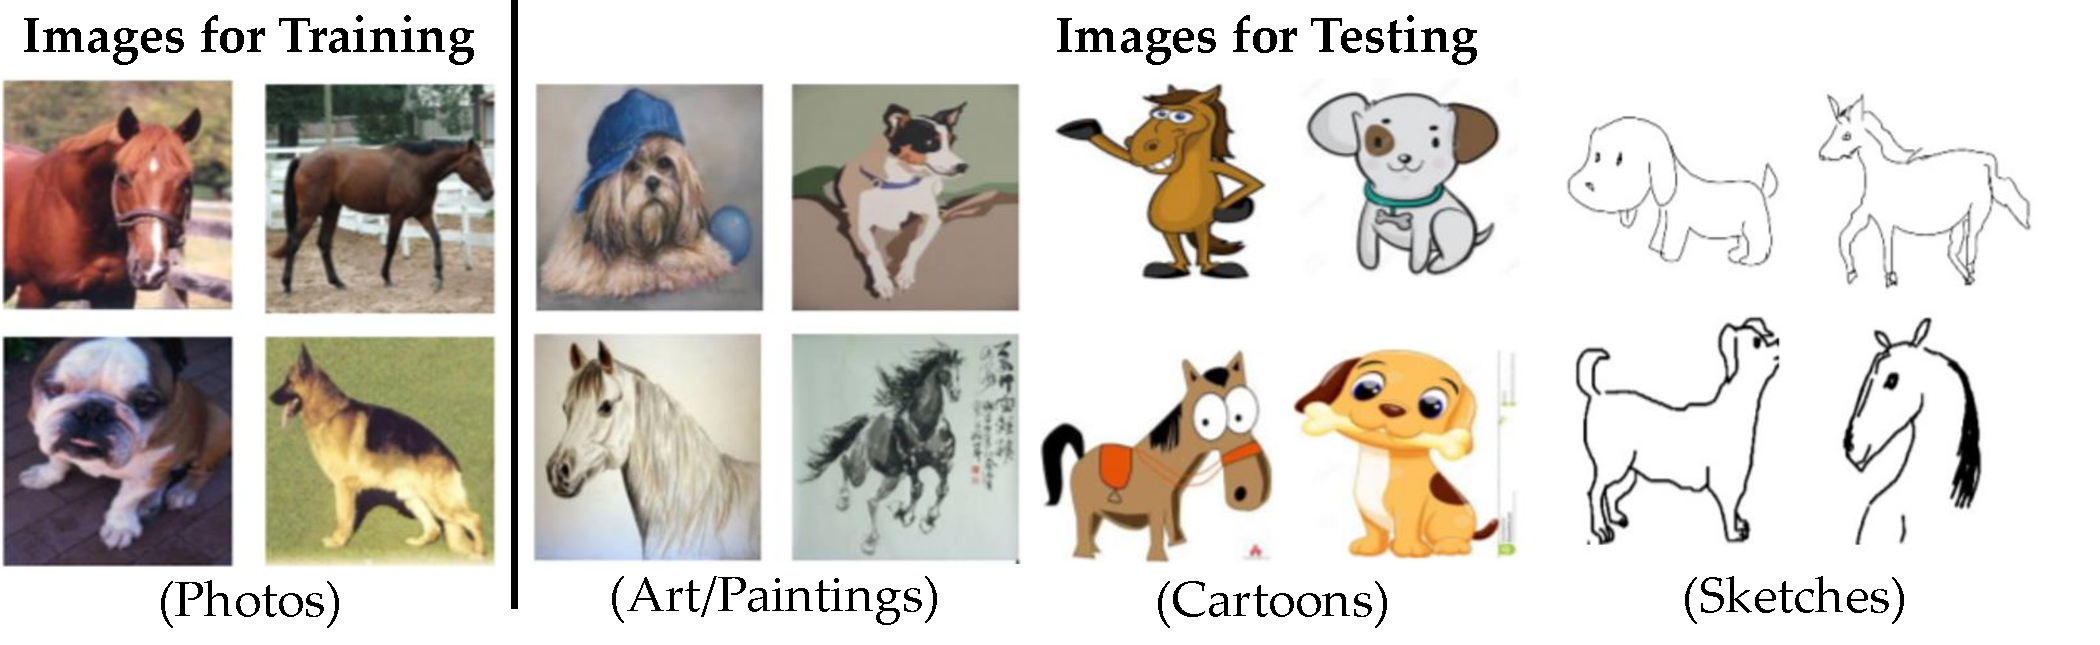
\includegraphics[width=\linewidth]{figures/pacs_styles.pdf}
    \caption{Illustration of the discrepancies between training data and real-world test data. A \textit{robust} image classifier is expected to perform reliably on a wide range of image styles and sources.
    Image adapted from \citet{li2017deeper}.
    }
    \label{fig:pacs_styles_introduction}
\end{figure}

\begin{figure}
    \centering
    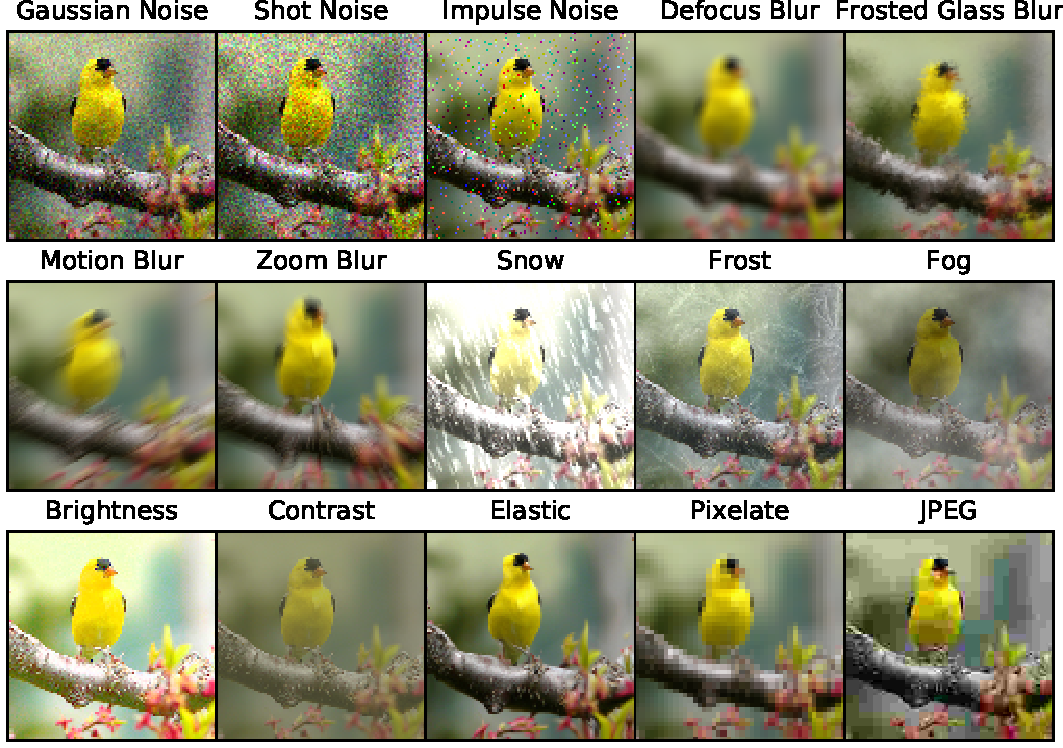
\includegraphics[width=\linewidth]{figures/distorted.pdf}
    \caption{
    Noise, blur, weather, or digital artifacts can also impact classifier performance at test-time.
    Image from \citet{hendrycks2018benchmarking}.
    }
    \label{fig:cifar_c_introduction}
\end{figure}
The answer to these questions, unfortunately is in the negative.
Although highly capable of learning from training data, recent studies show that neural networks are prone to failure on new test sets or under distribution shift~\citep{taori2020measuring}, natural corruptions~\citep{hendrycks2018benchmarking}, adversarial attacks~\citep{goodfellow2014explaining}, spurious correlations~\citep{beery2018recognition}, and many other types of ``unseen'' changes in test samples.
This shortcoming stems from the \textit{i.i.d.} assumption in statistical machine learning which guarantees good performance only on test samples that are drawn from an underlying distribution that is identical to the training dataset.

Consider the case of digit classification.
Digit recognition models trained on the black-and-white MNIST training images are almost perfect ($>99.5\%$ accuracy) on the corresponding \textit{i.i.d.} test set, yet their performance on colored digits and real-world digits from street number plates is only around $70\%$~\citep{xu2020robust}.
Although the accuracy of image classifiers on multiple datasets of real-world photographs such as ImageNet and CIFAR is above $90\%$, when these models are used for classifying other styles of images (such as cartoons, sketches, paintings, etc.)~\citep{venkateswara2017deep,li2017deeper} belonging to the same classes, a performance degradation is observed -- the accuracies are as low as $24\%$ for cartoons, $29\%$ for sketches, $64\%$ for paintings~\citep{nam2021reducing}, as shown in Figure~\ref{fig:pacs_styles_introduction}
There is also a large accuracy drop when models are tested on natural corruptions~\citep{hendrycks2018benchmarking} such as fog, snow, rain, noise, blur etc. or geometric perturbations such as rotation, translation, scaling~\citep{wong2020learning}, as illustrated in Figure~\ref{fig:cifar_c_introduction}.
In short, when models that have been trained in ``lab settings'' are tested in ``real-world settings'', the levee breaks, and we start getting a glimpse into the robustness of computer vision models. 
\textit{This thesis is about identifying such modes of failure, analyzing them, and providing solutions for improving model robustness.}

\section{Overview: Towards Robust Visual Understanding}
The recent findings about the brittleness and high sensitivity of models on real-world data pose a significant challenge to the practical adoption of computer vision models and their reliability in the real-world, especially when dealing with sensitive data such as biomedical and satellite imagery, personal information, private records, etc.
In this dissertation, I will address these shortcomings in the domains of image classification as well as multi-modal visual understanding \textit{a.k.a.} vision-and-language (V\&L).
My work complements the new innovations of the past decade, by studying their robustness and generalization capabilities.
This involves:
\begin{enumerate} 
    \item \textbf{identifying failure modes}, i.e., situations under which systems may fail, for perceptual tasks (such as image classification) and semantic tasks (such as visual question answering, visual reasoning, and image/video captioning),
    \item creating \textbf{evaluation and analysis tools} to diagnose failures, achieved by creating datasets for targeted evaluation, probing models with specific types of input perturbations, evaluating generalization under domain shift or across datasets, etc.
    \item \textbf{developing techniques} that provide greater robustness to mitigate the risks posed by such situations.
\end{enumerate}



%%%% AGAT %%%%
In Chapter~\ref{chap:agat}, we consider a setup where robustness is expected over an unseen test domain that is not i.i.d.\ but deviates from the training domain.
While this deviation may not be exactly known, its broad characterization is specified \textit{a} priori, in terms of attributes.
We propose an adversarial training approach which learns to generate new samples so as to maximize exposure of the classifier to the attributes-space, without having access to the data from the test domain.
Our approach enables deep neural networks to be robust against a wide range of naturally occurring perturbations.
We demonstrate the usefulness of the proposed approach by showing the robustness gains of deep neural networks trained using our adversarial training on MNIST, CIFAR-10, and a new variant of the CLEVR dataset.
This work was published as a conference paper in AAAI 2021~\citep{gokhale2021attribute}.

To be successful in single source domain generalization, maximizing diversity of synthesized domains has emerged as one of the most effective strategies. Many of the recent successes have come from methods that pre-specify the types of diversity a model is exposed to during training so that it can ultimately generalize well to new domains. However, na\"ive diversity based augmentations do not work effectively for domain generalization either because they cannot model large semantic shifts, or the span of transforms that are pre-specified, do not cover the semantic shifts commonly occurring in domain generalization. 
%
%
%
%

%%%% ALT %%%%
To address this issue, in Chapter~\ref{chap:alt}, we present a novel framework that uses adversarially learned transformations (ALT) using a neural network to model plausible, yet hard image transformations that fool the classifier. This network is randomly initialized for each batch and trained for a fixed number of steps to maximize classification error. 
With extensive empirical analysis, we find that this new form of adversarial transformations achieve both objectives of diversity and hardness together, outperforming all existing techniques on competitive benchmarks for single source domain generalization. 
We also show that ALT can naturally work with existing diversity modules to produce highly distinct, and large transformations of the source domain leading to state-of-the-art performance.
This work is currently under review at CVPR 2022.
%
%
%
%

%%%% VQALOL %%%%
In Chapter~\ref{chap:vqalol} we start our foray into multi-modal vision-and-language tasks.
Multi-modal tasks involving both vision and language (V\&L) inputs, such as visual question answering (VQA), open up many more types of domain discrepancies that can affect model performance of test time.
For the VQA task, given an image and a question about it, models are trained to predict the answers to those questions.
In VQA-LOL, we discovered that existing VQA models fail when logical transformations such as negation, conjunction, and disjunction are introduced in the questions.
This surprising finding led us to develop a data augmentation tool that allows us to produce logical combinations of multiple questions in the source dataset, and a training objective that is based on Frechet inequalities to guide the predicted probabilities of answers to questions with negation, conjunction, and disjunction.
Thus, given a known transformation between source and target domains, we developed a method that can leverage data augmentation for improving robustness of VQA models.
This work was published as a conference paper in ECCV 2020~\citep{gokhale2020vqa}.
%
%
%
%

%%%% MUTANT %%%%
The work on VQA-LOL spawned off two additional projects: the first, VQA-MUTANT is about a data augmentation strategy to address changing priors between train and test datasets.
In this paper, we make use of simple image transformations which remove objects or change their colors, in addition to the logical transformations developed above. Empirical results  on the VQA-CP challenge~\citep{agrawal2018don} show that this method achieves robustness under changing question-answer priors (i.e.~when the conditional probability of answers given a question type varies between train and test domains).
This work was published as a conference paper in EMNLP 2020~\citep{gokhale2020mutant}.
%
%
%
%

%%% SDRO %%%%
The problem of logical and linguistic brittleness is not limited to VQA.
In Chapter~\ref{chap:sdro}, we consider the task of vision-and-language inference (VLI), i.e. predicting whether an input sentence is \texttt{True} or \texttt{False} for a given image or video.
We define a set of linguistic transformations called ``SISP'' that contain semantics-inverting as well as semantics-preserving text transformations, such as negation, synonyms, antonyms, paraphrasing.
Analysis of VLI models using SISP transformations reveals their brittleness, especially under semantics-inverting phenomena.
While data augmentation techniques have been designed to mitigate against these failure modes, methods that can integrate this knowledge into the training pipeline remain under-explored.
We present \textbf{SDRO},
% \footnote{Code and data will be released upon publication.}
% % \footnote{\href{https://github.com/ASU-APG/VLI_SDRO}{\footnotesize\url{https://github.com/ASU-APG/VLI_SDRO}}}, 
a model-agnostic method that utilizes a set linguistic transformations in a distributed robust optimization setting, along with an ensembling technique to leverage these transformations during inference.
SDRO also allows us to learn in low-resource settings, serving as a smart data augmentation tool -- SDRO models trained only with $80\%$ of the original dataset outperform existing state-of-the-art which utilizes the entire dataset.
This work is currently under review at ACL 2022, and is available as a preprint~\citep{gokhale2021semantically}.
Shortly after, Neeraj Varshney led a project that constructed a larger set of transformations for unsupervised learning for the text-only task of natural language inference. I am third author for this paper, which is currently under review and available as a preprint~\citep{varshney2021unsupervised}.

% Chapter~\ref{sec:collabs} is a compendium of robustness and generalization study done as part of collaboration with Pratyay Banerjee who was the first author for these papers.
% While Pratyay has discussed these ideas on weak supervision from synthetic data and self-supervised training at length in his thesis, in this chapter, I will briefly discuss how model robustness in visual question answering is affected when trained with weak supervision.


\vspace*{\fill}
\paragraph{Disclosure of Funding Sources.}
Work done at ASU has been funded through grants from
National Science Foundation (grants \#1816039, \#1750082, 
Defence Advanced Research Projects Agency (SAIL-ON program \#W911NF2020006, KAIROS program ), 
and Office of Naval Research Research grant \#00014-20-1-2332.
My work as an intern at Lawrence Livermore National Laboratory was performed under the auspices of the U.S. Department of Energy under contract DE-AC52-07NA27344.
The views and opinions of the authors expressed herein do not necessarily state or reflect those of the funding agencies and employers.

% Deep neural networks have emerged as a widely popular architectural choice for modeling tasks in multiple domains such as (but not limited to) computer vision~\citep{yuille2021deep} and natural language processing~\citep{hochreiter1997long,vaswani2017attention}.
% Although highly capable of learning from training data, recent studies show that neural networks are prone to failure on new test sets or under distribution shift~\citep{taori2020measuring}, natural corruptions~\citep{hendrycks2018benchmarking}, adversarial attacks~\citep{goodfellow2014explaining}, spurious correlations~\citep{beery2018recognition}, and many other types of ``unseen'' changes in test samples.
% This shortcoming stems from the \textit{i.i.d.} assumption in statistical machine learning which guarantees good performance only on test samples that are drawn from an underlying distribution that is identical to the training dataset.
% For instance, digit recognition models trained on the black-and-white MNIST training images are almost perfect ($>99.5\%$ accuracy) on the corresponding \textit{i.i.d.} test set, yet their performance on colored digits and real-world digits from street number plates is only around $70\%$.
% Similarly, state-of-the-art NLP models have been shown to fail when negation is introduced in the input~\citep{kassner2020negated}.
% These findings pose a significant challenge to the practical adoption of computer vision models and their reliability in the real-world, especially when dealing with sensitive data such as biomedical and satellite imagery or other mission-critical applications in space exploration or drug discovery.

% My work addresses these shortcomings in the domain of 
% \begin{enumerate}[label=(\textbf{\Roman*}),nosep,noitemsep] % (a), (b), (c), ...
%     \item image classification, and 
%     \item multi-modal tasks (vision+language).
% \end{enumerate}
% The focus of my thesis is to identify the various situations under which machine learning models may fail while making predictions for tasks (\textbf{I}) or (\textbf{II}), and to develop machine learning techniques to mitigate risks posed therein.
% These can be categorized as:
% \begin{enumerate}[label=(\textbf{\Alph*}),nosep,noitemsep]
%     \item domain shift -- i.e.~when the training domain $\mathcal{D}$ and target test domain $\mathcal{D}^\prime$ are not identical -- for instance, a trainind domain with black-and-white digits, and target domain with real-world colored digits.
%     \item local perturbations -- i.e.~situations in which small perturbations such as noise and corruptions are encountered in the inputs at test time.
% \end{enumerate} 
% The choice of solution for \textbf{(A)} depends on how much information about the target domain is available during training.
% In cases when labeled target datasets are available, the best bet would be to include such labeled input-output pairs in the training dataset.
% When unlabeled target samples are available, solutions fall under the umbrella term of \textit{domain adaptation}, and seek to utilize unlabeled images to learn an invariant feature space.
% However when no explicit samples (either labeled or unlabeled) are available, the problem becomes that of \textit{domain generalization}.
% When only a single source of training data is available, this is a very challenging problem because of the limited information available to train the model with just a single source.

